%
%===============>>  ГРУППА 11-1 МОДУЛЬ 4  <<=============
%
\setmodule{4}
%
%===============>>  Занятие 1  <<===============
%
\begin{class}[number=1]
	\begin{listofex}
		\item Пусто
	\end{listofex}
\end{class}
%
%===============>>  Занятие 2  <<===============
%
%\begin{class}[number=2]
%	\begin{listofex}
%		\item Пусто
%	\end{listofex}
%\end{class}
%
%===============>>  Домашняя работа 1  <<===============
%
%\begin{homework}[number=1]
%	\begin{listofex}
%		\item Пусто
%	\end{listofex}
%\end{homework}
%
%===============>>  Занятие 3  <<===============
%
%\begin{class}[number=3]
%	\begin{listofex}
%		\item Пусто
%	\end{listofex}
%\end{class}
%
%===============>>  Занятие 4  <<===============
% смещение на одно занятие с прошлого месяца
%\begin{class}[number=4]
%	\begin{listofex}
%		\item Пусто
%	\end{listofex}
%\end{class}
%
%===============>>  Домашняя работа 2  <<===============
%
%\begin{homework}[number=2]
%	\begin{listofex}
%
%	\end{listofex}
%\end{homework}
%
%===============>>  Занятие 5  <<===============
% смещение на одно занятие с прошлого месяца
\begin{class}[number=5]
	\begin{listofex}
		\item
		\begin{minipage}[t]{0.67\textwidth}
			На рисунке изображён график функции вида \(f(x)=\dfrac{k}{x}+a\). Найдите, при каком значение \(x)\) значение функции равно \(0,8\).
		\end{minipage}
		\begin{minipage}[c]{0.25\textwidth}
			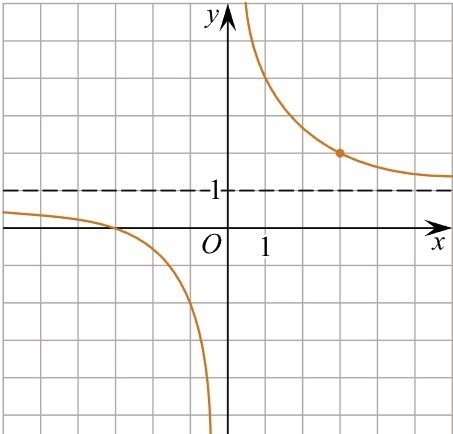
\includegraphics[align=t, width=\textwidth]{pics/G101M4C5-1.jpg}
		\end{minipage}
		\item
		\begin{minipage}[t]{0.67\textwidth}
			На рисунке изображён график функции вида \(f(x)=\dfrac{a}{x+b}+c\), где числа \(a, b, c\) --- целые. Найдите \(f(4)\).
		\end{minipage}
		\begin{minipage}[c]{0.25\textwidth}
			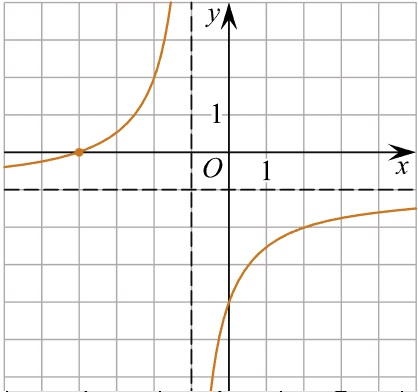
\includegraphics[align=t, width=\textwidth]{pics/G101M4C5-3.jpg}
		\end{minipage}
		\item
		\begin{minipage}[t]{0.67\textwidth}
			На рисунке изображён график функции вида \(f(x)=\dfrac{ax+b}{x+c}\), где числа \(a, b, c\) --- целые. Найдите \(a\).
		\end{minipage}
		\begin{minipage}[c]{0.25\textwidth}
			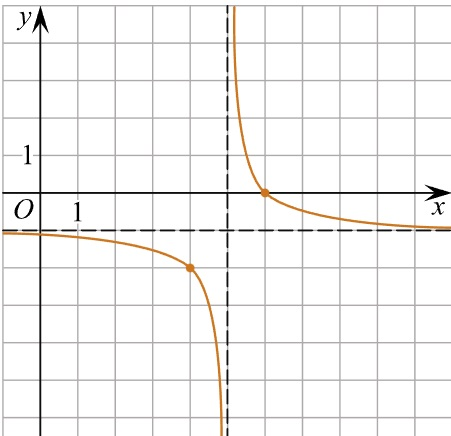
\includegraphics[align=t, width=\textwidth]{pics/G101M4C5-5.jpg}
		\end{minipage}
		\item
		\begin{minipage}[t]{0.67\textwidth}
			На рисунке изображён график функции вида \(f(x)=\dfrac{a}{x+b}+c\), где числа \(a, b, c\) --- целые. Найдите \(f\left(\dfrac{1}{3}\right)\).
		\end{minipage}
		\begin{minipage}[c]{0.25\textwidth}
			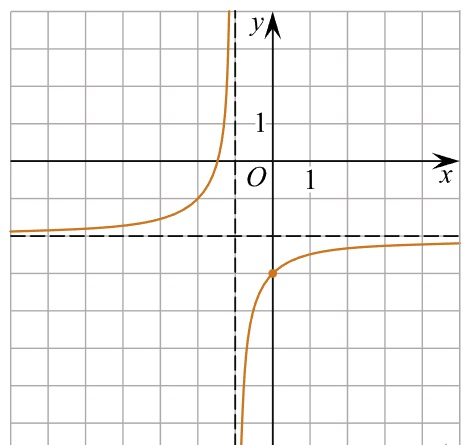
\includegraphics[align=t, width=\textwidth]{pics/G111M4C5-1.jpg}
		\end{minipage}
		\item
		\begin{minipage}[t]{0.62\textwidth}
			На рисунке изображён график функции вида \(f(x)=\dfrac{a}{x+b}+c\), где числа \(a, b, c\) --- целые. Найдите \(-3\).
		\end{minipage}
		\begin{minipage}[c]{0.35\textwidth}
			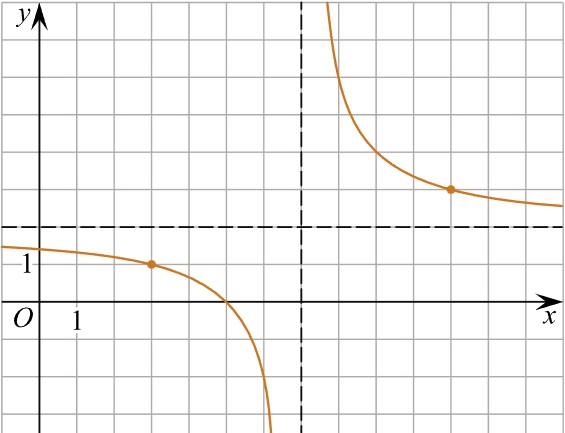
\includegraphics[align=t, width=\textwidth]{pics/G111M4C5-2.jpg}
		\end{minipage}
		\item
		\begin{minipage}[t]{0.76\textwidth}
			На рисунке изображён график функции вида \(f(x)=ax-|bx+c|+d\), где числа \(a, b, c, d\) --- целые. Найдите корень уравнения \(ax+d=0\).
		\end{minipage}
		\begin{minipage}[c]{0.17\textwidth}
			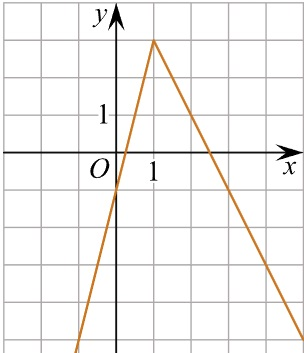
\includegraphics[align=t, width=\textwidth]{pics/G111M4C5-3.jpg}
		\end{minipage}
		\item
		\begin{minipage}[t]{0.76\textwidth}
			На рисунке изображён график функции вида \(f(x)=ax+|bx+c|+d\), где числа \(a, b, c, d\) --- целые. Найдите корень уравнения \(ax+d=10\).
		\end{minipage}
		\begin{minipage}[c]{0.15\textwidth}
			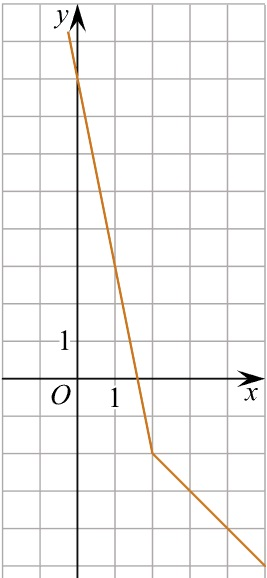
\includegraphics[align=t, width=\textwidth]{pics/G111M4C5-4.jpg}
		\end{minipage}
		\item
		\begin{minipage}[t]{0.76\textwidth}
			На рисунке изображён график функции вида \(f(x)=ax+|bx+c|+d\), где числа \(a, b, c, d\) --- целые. Найдите корень уравнения \(bx+c=0\).
		\end{minipage}
		\begin{minipage}[c]{0.15\textwidth}
			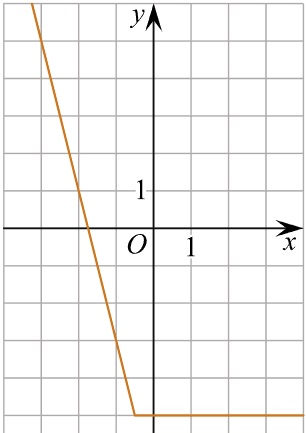
\includegraphics[align=t, width=\textwidth]{pics/G111M4C5-5.jpg}
		\end{minipage}
		\item
		\begin{minipage}[t]{0.76\textwidth}
			На рисунке изображён график функции вида \(f(x)=ax+|bx+c|+d\), где числа \(a, b, c, d\) --- целые. Найдите корень уравнения \(ax+d=0\).
		\end{minipage}
		\begin{minipage}[c]{0.15\textwidth}
			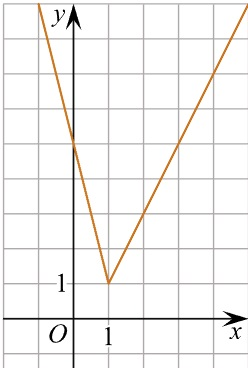
\includegraphics[align=t, width=\textwidth]{pics/G101M4C5-6.jpg}
		\end{minipage}
		\item
		\begin{minipage}[t]{0.76\textwidth}
			На рисунке изображён график функции вида \(f(x)=ax+|bx+c|+d\), где числа \(a, b, c, d\) --- целые. Найдите корень уравнения \(ax+d=19\).
		\end{minipage}
		\begin{minipage}[c]{0.15\textwidth}
			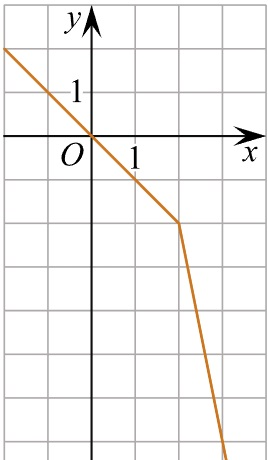
\includegraphics[align=t, width=\textwidth]{pics/G101M4C5-9.jpg}
		\end{minipage}
	\end{listofex}
\end{class}
%
%===============>>  Домашняя работа 3  <<===============
%
%\begin{homework}[number=2]
%	\begin{listofex}
%
%	\end{listofex}
%\end{homework}
%\newpage
%\title{Подготовка к проверочной работе}
%\begin{listofex}
%	
%\end{listofex}
%
%===============>>  Занятие 7  <<===============
%
%\begin{class}[number=7]
%	\begin{listofex}
%	
%	\end{listofex}
%\end{class}
%
%===============>>  Провечная работа  <<===============
%
%\begin{exam}
%	\begin{listofex}
%	
%	\end{listofex}
%\end{exam}